% !TEX encoding = UTF-8 Unicode

\documentclass[a4paper]{article}

\usepackage{color}
\usepackage{url}
\usepackage[T2A]{fontenc} % enable Cyrillic fonts
\usepackage[utf8]{inputenc} % make weird characters work
\usepackage{graphicx}
\usepackage[letterpaper,top=2cm,bottom=2cm,left=3cm,right=3cm,marginparwidth=1.75cm]{geometry}

\usepackage[english,serbian]{babel}
%\usepackage[english,serbianc]{babel} %ukljuciti babel sa ovim opcijama, umesto gornjim, ukoliko se koristi cirilica

\usepackage[unicode]{hyperref}
\hypersetup{colorlinks,citecolor=green,filecolor=green,linkcolor=blue,urlcolor=blue}

%\newtheorem{primer}{Пример}[section] %ćirilični primer
\newtheorem{primer}{Primer}[section]

\begin{document}


\title{Tehnološka singularnost\\ \small{Seminarski rad u okviru kursa\\Tehničko i naučno pisanje\\ Matematički fakultet}}

\author{Nikola Ahac\\ Dimitrije Petronijević\\ Mladen Radojević\\ Lazar Stošić}
\date{~Novembar 2022.}
\maketitle



\tableofcontents

\newpage

\section{Uvod}
\label{sec:uvod}
Tehnološku singularnost naučnici koriste kako bi označili hipotetički trenutak u budućnosti nakon koga će tehnološki napredak ubrzati I postati toliko komplikovan da će postati nedostupan našem razumevanju. Ovaj termin je prvobitno predložio američki matematičar I pisac naučne fantastike Vernor Vinge 1993. godine. Njegova ideja glasi ovako: Kada čovek stvori mašinu koja je pametnija od čoveka, budućnost će postati nepredvidiva, jer je nemoguće predviddeti ponašanje inteligencije koja je superiornija od čoveka. Vinge predviđa da do ovoga može doći negde u prvoj trećini 21. veka, negde između 2005. i 2003. godine. 

Ovo može dovesti do dva scenarija po našu civilizaciju. Prvi jeste scenario sličan onom u filmu “Matrix” u kome bi mašine pokušale da nas unište, a drugi jeste onaj optimističniji u kome bi ljudi i mašine živeli u miru. Mi ne možemo znati do čega će nas dovesti ovaj fenomen niti kada će taj trenutak doći.

\section{Eksplozija inteligencije}
Iako se tehnološki napredak ubrzava uvećini oblasti danas, on je dosta ograničen inteligencijom ljudskog mozga, koja se prema Pol R. Erlihu (eng. \textit{Paul R. Ehrlich}), nije značajno unapredila milenijumima.\cite{ref 1} Međutim napretkom informacioniih tehnologija i samih računara, u nekoj skorijoj budućnsti može se napraviti mašina koja je znatno inteligentnija od ljudi .

Ako bi se i konstruisala nadljudska inteligencija, bilo to poboljšanjem ljudske inteligencije ili stvaranjem nove veštačke inteligencije, to bi moglo dovesti do toga da se stvori mašina koja je sposobna da sama sebe nadogradjuje, i kroz vreme bi taj proces postajao sve brži i brži do trenutka kada više ne bi mogao da se isprati.

Pojam \textbf{„Eksplozije inteligencije“} je 1965. prvi put pomenuo I.J. Good\cite{ref 2}

\begin{itemize}
\item Neka ultrainteligentna mašina bude definisana kao mašina koja može daleko nadmašiti sve intelektualne aktivnosti bilo kog čoveka koliko god da je pametan. Pošto je projektovanje mašina jedna od ovih intelektualnih aktivnosti, ultrainteligentna mašina bi mogla da dizajnira još bolje mašine; tada bi nesumnjivo došlo do „eksplozije inteligencije“ i inteligencija čoveka bi ostala daleko iza. Tako je prva ultrainteligentna mašina poslednji izum koji čovek treba da napravi, pod uslovom da je mašina dovoljno poslušna da nam kaže kako da je držimo pod kontrolom.
\end{itemize} 
\section{Kako i kada će doći do singularnosti}	
\label{sec:kakoikada}
To kako i kada će doći do singularnost niko ne može sa sigurnošću tvrditi, postoje mnoge pretpostavke i ideje, ali se takva stvar jednostavno ne može predvideti.

U daljem tekstu će biti predstavljeno par takvih ideja.
\subsection{Pojava superingelencije}

Superinteligencija, hiperinteligencija ili nadljudska inteligencija je pojam koji se odnosi na neku vrstu veštačke inteligencije koja daleko nadmašuje inteligenciju ljudskog mozga.  John von Neumann, Vernor Vinge i Rej Kurzwelli smatraju da je današnjem čoveku nemoguće da predvidi kakve će posledice po njega imati nastanak „Super inteligencije“.
Međutim neki tehnološki prognostičari i istraživači se ne slažu oko toga kada će i da li će ljudska inteligencija biti nadmašena.  Neki tvrde da će napredak u veštačkoj inteligenciji verovatno rezultirati opštim sistemima rasuđivanja koji zaobilaze ljudska kognitivna ograničenja. Drugi veruju da će ljudi evoluirati ili direktno modifikovati svoju biologiju kako bi postigli radikalno veću inteligenciju.\cite{ref 3}
Brojni scenariji studija budućnosti kombinuju ove mogućnosti, sugerišući da će se ljudi verovatno povezati sa računarima ili preneti svoje umove na računare, na način koji omogućava značajno povećanje inteligencije. Knjiga \textbf{The Age of Em} od Robina Hansona opisuje budućnost u kojoj se pojavljuju ljudski mozgovi umesto ili na putu do pojave superinteligencije.

\subsection{Singularnost bez veštačke inteligencije}

Neki naučnici koriste „singularnost“ na širi način tako što upućuju na bilo kakve radikalne promene u našem društvu izazvane novim tehnologijama kao što je molekularna nanotehnologija,\cite{ref 4} iako Vinge i drugi naučnici posebno navode da bez superinteligencije, takve promene se ne bi kvalifikovale kao prava singularnost.

\subsection{Brza superinteligencija}
Brza superinteligencija opisuje veštačku inteligenciju koja može da funkcioniše kao ljudski um, samo dosta brže. Na primer, sa milion puta povećanom brzinom obrade informacija u odnosu na ljude, subjektivna godina bi prošla za 30 fizičkih sekundi. Takva razlika u brzini obrade informacija mogla bi da pokrene singularnost.

\section{Verovatnoća da će doći do singularnosti}	
\label{sec:verovatnoća}
Nekoliko istaknutih tehnologa i akademika je diskutovalo o mogućnosti da se singularnost ostvari. 

Većina njih predlaže da do singularnosti može doći na jedan od dva načina: veštačkom inteligencijom i amplifikacijom ljudskog mozga, za koju su neke od predloženih metoda bioinženjering, genetski inženjering, AI asistenti, različite vrste droga, direktna veza mozga i računara, kao i "upload-ovanje" mozga na računar. Računajući da se konstantno radi na istraživanju ovakvih grana, mogućnost da dođemo do singularnosti se samo povećava. 

Tri glavna faktora koji utiču na ostvarivanje singularnosti su: \cite{mog-2}
\begin{itemize}
\item Prvi, ubrzavajući, faktor su poboljšivači inteligencije, koji se konstantno nadograđuju na svoje predhodnike 
\item Drugi, nasuprot prvom, je usporavajući faktor i on je otežavanje napretka time što je tehnologija sve naprednija. U jednom momentu će se možda doći da će komplikacije u razvoju prevazići potencijalni napredak inteligencije
\item Treći, isto usporavajući, je eventualna fizička granica, gde zakoni fizike neće dozvoljavati dalji napredak  
\end{itemize} 
U online anketi iz 2017. godine, na pitanje koliko je verovatno da dođe do eksplozije inteligencije, 12\% ispitanika je reklo da će "vrlo verovatno" doći do iste, 17\% ispitanika je reklo "verovatno", 21\% ispitanika je reklo "možda", 24\% ispitanika je reklo "malo verovatno", a 26\% ispitanika je reklo da je to "skoro nemoguće". \cite{mog-3}

\subsection{Razvoj brzine tehnološkog napretka}

Murov zakon (eng.~{\em Moore's law}) je opažanje da se broj tranzistora po jedinici prostora duplira na svake dve godine (grafik tog razvoja je prikazan na slici \ref{fig:grafik}). 

Analogija Murovom zakonu je da ako bi za prvo dupiranje brzine hardvera računara trebalo \textbf{18 meseci}, sa sledeće bi trebalo \textbf{9}, posle čega bi trebalo \textbf{četiri}, pa \textbf{dva}, \textbf{jedan} i tako dalje dok se eventualno ne bi došlo do neke gornje granice za brzinu.

Džef Hokins (eng.~{\em Jeff Hawkins}) je rekao da bi samopoboljšavajući računarski sistem eventualno došao do neke gornje granice računarske snage : "postoji granica koliko brzi i veliki računari mogu da postanu. U svakom slučaju, završićemo na istoj tački, možda samo malo brže. Ne bi došlo do singularnosti". \cite{mog-5}

\begin{figure}[h!]
\begin{center}
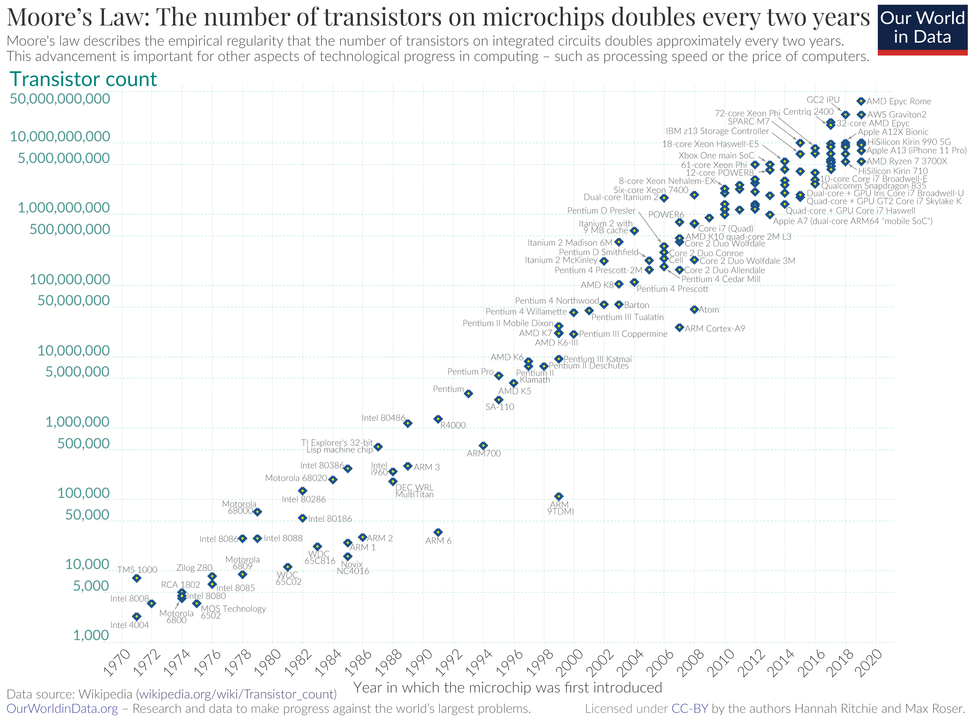
\includegraphics[scale=0.35]{moore.png}
\end{center}
\caption{Murov zakon}
\label{fig:grafik}
\end{figure}

Eksponencijalni napredak predložen u Murovom zakonu se koristi kao jedan od glavnih pokazatelja da u skorijoj budućnosti očekujemo pojavu singularnosti.

Rej Kurcvail (eng.~{\em Jeff Hawkins}) predlaže zakon o ubrzanom povratku, generalizujuću Murov zakon na celokupnu tehnologiju i govori o tome da se brzina tehnološkog razvoja eksponencijalno povećava. Taj zakon primenjuje i na tehnologije kao što su materijalna, medicinska i druge.

Kurcvail takođe veruje da će se singularnost desiti do 2045. godine, jer smatra da će tada veštačka inteligencija nadjačati ukupnu sumu moždanog kapaciteta celog čovečanstva.


\subsection{Razvoj algoritama}

Neke tehnologije, kao 'seed AI', imaju potencijal da se ne samo ubrzaju, već i da poboljšaju svoju efikasnost promenom sopstvenog izvornog koda. 
Ovaj mehanizam se od čistog povećanja brzine izvršavanja razlikuje u dva pogleda.

Prvo, za njega nije potreban spoljni uticaj. Za razliku od hardverskog ubrzavanja, gde je potreban bar neki nivo interakcije od strane čoveka, u ovom mehanizmu AI sam menja sopstveni kod.

Drugo, kao po Vernor Vindžovom (eng.~{\em Vernor Vinge}) viđenju singularnosti, ovaj pristup može biti vrlo nepredvidiv. \cite{mog-8}

\subsection{Kritike}

Neki kritičari, kao Hjubert Drejfus (eng.~{\em Hubert Dreyfus}) tvrde da računari i mašine ne mogu dostići nivo ljudske inteligencije, dok neki kao fizičar Stiven Hoking (eng.~{\em Stephen Hawking}) tvrde da je definicija inteligencije zanemarljiva ukoliko je krajnji rezultat isti. 

Martin Ford u svojoj knjzi \textbf{"The Lights in the Tunnel: Automation, Accelerating Technology and the Economy of the Future"} predlaže "tehnološki paradoks", gde tvrdi da do singularnosti neće doći, zato što bi ona dovela do masovne nezaposlenosti i smanjene trgovinske potražnje, jer bi se pokazala efikasnijom od radnika, što bi za uzvrat dovelo do smanjene inicijative da se ulaže u iste tehnologije. \cite{mog-10}

\section{Potencijalni uticaj}
\label{sec:potencijalni_uticaj}
\hfill

Ogromne promene u stopi ekonomskog rasta su se dogodile u prošlosti zbog tehnološkog napredka. U odnosu na rast populacije, ekonomija se duplirala svakih \textbf{250,000 godina} od Paleolita do Neolitske revolucije. Nova, poljoprivredna ekonomija se duplirala na svakih \textbf{900 godina}, ovo je naravno ogromna razlika. Od Industrijske Revolucije pa na dalje, ekonomski učinak se duplirao na svakih \textbf{15 godina}. Kada bi superinteligencija izazvala sličnu revoluciju, bilo bi očekivano da se ekonomija duplira na nedeljnoj bazi čak.

\subsection{Nestabilnost i rizik}
\label{subsec:nestabilnost_i_rizik}
\hfill

Termin \textbf{"Tehnološka singularnost"} predstavlja ideju da se to može dogoditi uskoro. Naravno, mi kao ljudi ne možemo da predpostavimo kada će to biti, niti da li će se to uopšte desiti. Ne bi mogli ni da pretpostavimo kako bi taj svet zapravo izgledao. 

Štaviše, nije sigurno ni da li bi ta revolucija bila dobra za ljudski rod, možda bi baš to predstavljalo kraj društva. Dobar broj kompanija pokušava da glavni cilj veštačke inteligencije uskladi sa ljudskim vrednostima na što bolji način, ne bi li stvorili veštačku inteligenciju koja je dobroćudna.

Fizičar Stiven Hoking (eng. \textit{Stephen Hawking}) je u 2014, rekao da \textbf{"Uspeh u stvaranju veštačke inteligencije bi bio najveći uspeh u ljudskoj istoriji. Nažalost, to bi veorovatno bio i poslednji, osim ako ne naučimo kako da izbegnemo rizike."}\cite{r2}

Berglas (eng. \textit{Anthony Berglas}) tvrdi da ne postoji nikakva evoluciona motivacija koja bi veštačku inteligenciju učinilo da bude prijateljski nastrojena. Evolucija nema nikakve težnje da stvori ishod koji ljudi žele. Veća je verovatnoća da se AI ponaša suprotno od onoga kako su ljudi planirali.

Elizer Judkovski (eng. \textit{Eliezer Yudkowsky}) tvrdi da su veće šanse da se kreira neprijateljski nastrojena veštačka inteligencija, umesto suprotne koja bi bila od velike pomoći i kojoj ljudi pokušavaju da se približe.

\subsection{Sledeći korak evolucije}
\label{subsec:sledeći_korak_evolucije}
\hfill

Dok je tehnološka jednakost viđena kao događaj koji se dešava tek tako od jednom, neki naučnici tvrde da je trenutna brzina evolucije perfektna takva kakva jeste.

Pojedini kažu da smo trenutno u sred velike evolucione promene koja spaja tegnologiju, biologiju i društvo. Tehnologija već predstavlja deo svakodnevnog života većine ljudi.

Članak \textit{Trends in Ecology \& Evolution}\cite{r3} iz 2016. tvrdi da "ljudi već prihvataju spoj tehnologije i biologije. Kada god se šetamo i razgovaramo telefonom, koristimo digitalno umešane službe koje omogućavaju taj razgovor. Verujemo veštačkoj inteligenciji čak i kada su naši životi u pitanju, dobar primer bi bio sistem za izbegavanje blokiranja kočnica u automobilima (eng. \textit{Antilock Braking System}), autopilotni mod u avionima i automobilima, itd."

\subsection{Brzina rasta broja digitalnih informacija}
\label{subsec:broj_digitalnih_informacija_}

\hfill

Broj digitalnih informacija koje su ljudi stvorili je skoro iste veličine kao broj bioloških informacija u biosferi. Od 1980-te pa sve do danas, broj digitalnih informacija se duplirao na svake 2.5 godine, i dostigao otprilike 5 zetabajta (eng. \textit{Zettabyte}) u 2014. godini (5x$10^{21}$ bajtova).

Biološki gledano, postoji 7.2 milijarde ljudi na planeti zemlji (članak iz 2014. godine), svaka osoba ima genom koji je sačinjen od 6.2 milijarde nukleotida. Pošto jedan bajt (eng. \textit{Byte}) može da predstavi 4 nukleotidna para, onda bi broj svih genoma svih osoba na planeti zemlji mogao da se približno odredi sa brojem 1x$10^{19}$. Poređenja radi, broj digitalnih informacija je 500 puta veći (5x$10^{21}$). Ukupna količina DNK parova sadržana u svim ćelijama na planeti zemlji je 5.3x$10^{37}$, što bi bilo tačno 1.325x$10^{37}$ bajtova.

Kada bi broj digitalnih informacija nastavio da raste trenutnim tempom od 30-38\% godišnje, broj DNK parova svih ćelija na planeti zemlji bi stigli za 110 godina. Ovo bi predstavilo dupliranje ukupnog broja informacija biosfere za samo 150 godina, što je nevorovatno kratko vreme za ovako velike brojeve.\cite{r6}







\section{Teško i lako poletanje AGI-a}
\label{sec:poletanje}
Kada i ako dođe do tehnološke singularnosti, postoje dva moguća scenarija, \textbf{teško poletanje} i \textbf {lako poletanje}.
Pod teškim poletanjem podrazumevamo veoma brzo i eksplozivno samopoboljšanje AGI-a, gde ono \textit{"preuzima kontrolu"} nad svetom toliko brzo(možda za nekoliko sati) da je ljudska interakcija i korekcija nemoguća. Kod lakog poletanja sa druge strane, veštačka inteligencija postaje moćnija od čoveka ali u manjem vremenskom intervalu (decenijama) što daje mogućnost čovečanstu da spreči ili bar preusmeri i interaguje sa ciljevima AGI-a tokom njegove evolucije.\cite{refe1}

Ramez Naam, Američki tehnolog i pisac naučne fantastike, se protivi teškom poletanju.On tvrdi da mi vec sad imamo primere rekurzivnog samo-poboljsavanja superinteligencija. Na primer, Intel je kompanija koja ima na milione CPU jezgara i a hiljade ljudskih umova, ali to nije dovelo do teškog poletanja, već do lakog poletanja u obliku Murovog zakona \cite{refe2}. Naam takođe tvrdi da složenost računara više inteligencije moze biti mnogo veća od linearne, čime i trud za evolucijom postaje eksponecijalno veći.\cite{refe3}

"Većina čestih scenarija teškog poletanja su kružna, jer se u svakom 0predpostavlja nadljudska mogućnost samo-poboljsavanja AGI-a na samom početku kao preduslov za bilo kakvo poletanje" veruje John Storrs Hall. Hall sugeriše da bi novoj veštačkoj inteligenciji bilo bolje da se specijalizuje u jednoj oblasti u kojoj je najefikasnija, a zatim da kupi preostale komponente sa tržišta, umesto da rekurzivno samo-poboljšava svoj hardver, softver i infrastrukturu, jer se kvalitet proizvoda na tržištu stalno poboljšava, a veštačka inteligencija bi imala poteškoća da održi korak sa najsavremenijom tehnologijom koju koristi ostatak sveta.\cite{refe4}

\section{Besmrtnost}
\label{sec:besmrtnost}
  U svojoj knjizi iz 2005.\textit {Singularnost je blizu}, Kurcvajl sugeriše da bi napredak medicine omogućio ljudima da zaštite svoja tela od efekata starenja, čineći očekivani životni vek neograničenim. 
  
  Kurzveil tvrdi da bi nam tehnološki napredak u medicini omoućio da kontinuirano popravljamo i zamenjujemo defektne komponente u našim telima, produžavajući život do neodređenog doba.
  
  Kurcveil dalje potkrepljuje svoj argument diskusijom o trenutnim dostignućima bioinženjeringa. Kurcveil predlaže somatsku gensku terapiju; nakon sintetičkih virusa sa specifičnim genetskim informacijama, sledeći korak bi bio da se ova tehnologija primeni na gensku terapiju, zamenjujući ljudsku DNK sintetizovanim genima.\cite{refe5}

  Prema teoretskom fizičaru  Richard Feynman-u, njegov nekadašnji student Albert Hibbs mu je predlozio korišćenje Feynman-ovih teoretskih mikromašina u okviru medicine. Hibbs je reako da određene mašine za preparvku bi se u budunosti mogle smanjiti na te veličine gde bi bilo moguće "progutati ih". Feyman je ovu ideju iskoristio u svom eseju \textit{ There's Plenty of Room at the Bottom.}\cite{refe6}
\section{Istorijat koncepta}
\label{sec:istorijat}

Marquis de Condorcet je bio prvi čovek koji je pretpostavio i matematički modelirao razvoj iteligencie i njen uticaj na čoveka u 18. veku. Njegovu ideju je potom prvi razvijo John W. Campbell u svojoj kratkoj priči\textit{ "The last evolution"} 1932. godine .\cite{refe7}

Stanislaw Lem je 1981. objavio svoj naučnofantastični roman Golem KSIV. Opisuje vojni kompjuter sa veštačkom inteligencijom (Golem KSIV) koji dobija svest i počinje da povećava sopstvenu inteligencija,krećuči se ka ličnoj tehnološkoj singularnosti.\cite{refe8}


Golem KSIV je prvobitno stvoren da pomogne svojim graditeljima u vođenju ratova, ali kako njegova inteligencija napreduje na mnogo viši nivo od ljudske, prestaje da bude zainteresovan za vojne zahteve jer smatra da im nedostaje unutrašnja logička doslednost.

Godine 1983, Vernor Vinge je u velikoj meri popularizovao Gudovu eksploziju obaveštajnih podataka u brojnim spisima, prvi put se na tu temu u štampanom izdanju u januarskom izdanju časopisa Omni 1983. godine. U ovom tekstu, Vinge je izgleda bio prvi koji je upotrebio termin „singularnost“ na način koji je bio posebno vezan za stvaranje inteligentnih mašina.\cite{refe9}

Godine 2000. Bill Joi, istaknuti tehnolog i suosnivač kompanije Sun Microsistems, izrazio je zabrinutost zbog potencijalnih opasnosti od singularnosti.\cite{refe10}

Kurcvajl je 2005. objavio Singularnost je blizu. Kurcvajlova kampanja za publicitet uključivala je nastup u The Daili Shov sa Džonom Stjuartom.\cite{refe11}

Godine 2007, Eliezer Iudkovski je sugerisao da su mnoge različite definicije koje su dodeljene „singularnosti“ međusobno nekompatibilne, a ne da se međusobno podržavaju. Na primer, Kurcvajl ekstrapolira trenutne tehnološke putanje mimo dolaska samopoboljšajuće veštačke inteligencije ili nadljudske inteligencije, za koju Judkovski tvrdi da predstavlja tenziju sa I. J. Goodovim predloženim diskontinuiranim porastom inteligencije i Vindžovom tezom o nepredvidljivosti.\cite{refe12}\cite{refe13}

Godine 2009. Kurcvajl i osnivač Ks-Prize Peter Diamandis objavili su osnivanje Univerziteta Singulariti, neakreditovanog privatnog instituta čija je navedena misija „da obrazuje, inspiriše i osnaži lidere da primenjuju eksponencijalne tehnologije za rešavanje velikih izazova čovečanstva“.[116] Gugl, Autodesk, ePlanet Ventures i grupa lidera tehnološke industrije, Univerzitet Singulariti se nalazi u NASA-inom istraživačkom centru Ames u Mauntin Vjuu, Kalifornija. Ova neprofitna organizacija vodi godišnji desetonedeljni diplomski program tokom leta koji pokriva deset različitih tehnologija i srodnih pravaca, kao i niz programa za rukovođenje tokom cele godine.\cite{refe14}


\section{Korist u politici}
\label{sec:politika}
2007. godine Zajednički ekonomski komitet Kongresa Sjedinjenih Američkih Država objavio je izveštaj o budućnosti nanotehnologije. Oni predviđaju značajne tehnološke i političke promene u srednjoročnoj budućnosti, uključujući moguću tehnološku singuarnost.\cite{refe15}\cite{refe16}\cite{refe17}

Bivši predsednik Sjedinjenih Američkih Država Barac Obama se pozvao jednom prilikom na tehnološku singularnost tokom jednog intervjua magazina \textit{Wired} 2016. godine.\cite{refe18}
\section{Zaključak}
\label{sec:zakljucak}
sadržaj kojeg smo se dotakli u ovom radu nije ni trunkica pravog potencijala beskonačnog samorazvića veštačke inteligencije i njene primene. Mi možemo samo da spekuličemo kada će doći do singularnosti, ali mnogi tvrde da, ako veštačka inteligencija nastavi da se razvija bryinom koju možemo da pratimo, moći ćemo da je pratimo i da utičemo na ishod i njen tok razvića. U slučaju da se AI alarmno razvije preko noći, niko neće moći da predvidi do kakvog će ishoda dovesti taj skok.

Možemo samo da se nadamo budućnosti u kojoj mašine neće preuzeti ulogu čoveka.

\addcontentsline{toc}{section}{Literatura}
\appendix

\iffalse
\bibliography{seminarski} 
\bibliographystyle{plain}
\fi

\begin{thebibliography}{9}

\bibitem{ref 1} Ehrlich, Paul. The Dominant Animal: Human Evolution and the Environment Archived 2018-10-08 at the Wayback Machine


 \bibitem{ref 2} Good, I. J. "Speculations Concerning the First Ultraintelligent Machine", Advances in Computers, vol. 6, 1965. Archived May 1, 2012, at the Wayback Machine
 
  \bibitem{ref 3} Vinge, Vernor. "The Coming Technological Singularity: How to Survive in the Post-Human Era" Archived 2018-04-10 at the Wayback Machine, in Vision-21: Interdisciplinary Science and Engineering in the Era of Cyberspace, G. A. Landis, ed., NASA Publication CP-10129, pp. 11–22, 1993.


\bibitem{ref 4} Sandberg, Anders. An overview of models of technological singularity Archived 2011-07-24 at the Wayback Machine

\bibitem{mog-2} Hanson, Robin (1998). \href{https://mason.gmu.edu/~rhanson/vc.html#hanson}{"Some Skepticism"}.

\bibitem{mog-3} Grace, Katja; Salvatier, John; Dafoe, Allan; Zhang, Baobao; Evans, Owain (24 May 2017). "When Will AI Exceed Human Performance? Evidence from AI Experts"

\bibitem{mog-5} https://spectrum.ieee.org/tech-luminaries-address-singularity

\bibitem{mog-8} Eliezer S. Yudkowsky. "Power of Intelligence"

\bibitem{mog-10}
\href{https://www.nytimes.com/2011/03/05/science/05legal.html}{"Armies of Expensive Lawyers, Replaced by Cheaper Software"}.

\bibitem{r2}
Stephen Hawking: "Success in creating AI would be the biggest event in human history. Unfortunately, it might also be the last, unless we learn how to avoid the risks."

\bibitem{r3}
\href{https://www.sciencedirect.com/science/article/abs/pii/S0169534703003458}{"Trends in Ecology \& Evolution"}


\bibitem{r6}
\href{https://escholarship.org/uc/item/38f4b791}{Information in the Biosphere: Biological and Digital Worlds}

\bibitem{refe1}  Bugaj, Stephan Vladimir, and Ben Goertzel. "Five ethical imperatives and their implications for human-AGI interaction." Dynamical Psychology (2007).

\bibitem{refe2}Naam, Ramez (2014). "The Singularity Is Further Than It Appears". Archived from the original on 17 May 2014. 

\bibitem{refe3} Naam, Ramez (2014). "Why AIs Won't Ascend in the Blink of an Eye - Some Math"
\bibitem{refe4} Hall, J. Storrs (2008). "Engineering Utopia". Artificial General Intelligence, 2008: Proceedings of the First AGI Conference.

\bibitem{refe5} \textit{The singularity Is Near p. 215.-216.}

\bibitem{refe6} Feynman, Richard P. (December 1959). "There's Plenty of Room at the Bottom".

\bibitem{refe7}Prasad, Mahendra (2019). "Nicolas de Condorcet and the First Intelligence Explosion Hypothesis"

\bibitem{refe8} Ulam, Stanislaw (May 1958). "Tribute to John von Neumann"

\bibitem{refe9} Dooling, Richard. Rapture for the Geeks: When AI Outsmarts IQ

\bibitem{refe10}Joy, Bill (April 2000), "Why The Future Doesn't Need Us", Wired Magazine, Viking Adult, vol. 8, no. 4, ISBN 978-0-670-03249-5, archived from the original on 2009-02-05, retrieved 2007-08-07

\bibitem{refe11} Episode dated 23 August 2006 at IMDb

\bibitem{refe12}Yudkowsky, Eliezer. The Singularity: Three Major Schools Archived 2018-10-01 at the Wayback Machine

\bibitem{refe13}Sandberg, Anders. "An overview of models of technological singularity." Roadmaps to AGI and the Future of AGI Workshop, Lugano, Switzerland, March. Vol. 8. 2010.

\bibitem{refe14} Singularity University Archived 2021-02-15 at the Wayback Machine at its official website

\bibitem{refe15} Guston, David H. (14 July 2010). Encyclopedia of Nanoscience and Society. SAGE Publications. ISBN 978-1-4522-6617-6. Archived from the original on 15 February 2021. Retrieved 4 November 2016.

\bibitem{refe16}"Nanotechnology: The Future is Coming Sooner Than You Think". Joint Economic Committee. March 2007. Archived from the original on 2021-02-15. Retrieved 2012-04-29.

\bibitem{refe17} "Congress and the Singularity". Archived from the original on 2021-02-15. Retrieved 2016-11-04.

\bibitem{refe18}Dadich, Scott (12 October 2016). "Barack Obama Talks AI, Robo Cars, and the Future of the World".

\bibitem{laski2009software} J. Laski and W. Stanley. \emph{Software Verification and Analysis}. Springer- Verlag, London, 2009.

\bibitem{gcc} Free Software Foundation. GNU gcc, 2013. on-line at: http://gcc. gnu.org/.

\bibitem{haltingproblem} A. M. Turing. \emph{On Computable Numbers, with an application to the Entscheidungsproblem}. Proceedings of the London Mathematical Society, 2(42):230–265, 1936.

\end{thebibliography}



\end{document}
